\documentclass[twoside]{book}

% Packages required by doxygen
\usepackage{fixltx2e}
\usepackage{calc}
\usepackage{doxygen}
\usepackage[export]{adjustbox} % also loads graphicx
\usepackage{graphicx}
\usepackage[utf8]{inputenc}
\usepackage{makeidx}
\usepackage{multicol}
\usepackage{multirow}
\PassOptionsToPackage{warn}{textcomp}
\usepackage{textcomp}
\usepackage[nointegrals]{wasysym}
\usepackage[table]{xcolor}

% Font selection
\usepackage[T1]{fontenc}
\usepackage[scaled=.90]{helvet}
\usepackage{courier}
\usepackage{amssymb}
\usepackage{sectsty}
\renewcommand{\familydefault}{\sfdefault}
\allsectionsfont{%
  \fontseries{bc}\selectfont%
  \color{darkgray}%
}
\renewcommand{\DoxyLabelFont}{%
  \fontseries{bc}\selectfont%
  \color{darkgray}%
}
\newcommand{\+}{\discretionary{\mbox{\scriptsize$\hookleftarrow$}}{}{}}

% Page & text layout
\usepackage{geometry}
\geometry{%
  a4paper,%
  top=2.5cm,%
  bottom=2.5cm,%
  left=2.5cm,%
  right=2.5cm%
}
\tolerance=750
\hfuzz=15pt
\hbadness=750
\setlength{\emergencystretch}{15pt}
\setlength{\parindent}{0cm}
\setlength{\parskip}{3ex plus 2ex minus 2ex}
\makeatletter
\renewcommand{\paragraph}{%
  \@startsection{paragraph}{4}{0ex}{-1.0ex}{1.0ex}{%
    \normalfont\normalsize\bfseries\SS@parafont%
  }%
}
\renewcommand{\subparagraph}{%
  \@startsection{subparagraph}{5}{0ex}{-1.0ex}{1.0ex}{%
    \normalfont\normalsize\bfseries\SS@subparafont%
  }%
}
\makeatother

% Headers & footers
\usepackage{fancyhdr}
\pagestyle{fancyplain}
\fancyhead[LE]{\fancyplain{}{\bfseries\thepage}}
\fancyhead[CE]{\fancyplain{}{}}
\fancyhead[RE]{\fancyplain{}{\bfseries\leftmark}}
\fancyhead[LO]{\fancyplain{}{\bfseries\rightmark}}
\fancyhead[CO]{\fancyplain{}{}}
\fancyhead[RO]{\fancyplain{}{\bfseries\thepage}}
\fancyfoot[LE]{\fancyplain{}{}}
\fancyfoot[CE]{\fancyplain{}{}}
\fancyfoot[RE]{\fancyplain{}{\bfseries\scriptsize Generated by Doxygen }}
\fancyfoot[LO]{\fancyplain{}{\bfseries\scriptsize Generated by Doxygen }}
\fancyfoot[CO]{\fancyplain{}{}}
\fancyfoot[RO]{\fancyplain{}{}}
\renewcommand{\footrulewidth}{0.4pt}
\renewcommand{\chaptermark}[1]{%
  \markboth{#1}{}%
}
\renewcommand{\sectionmark}[1]{%
  \markright{\thesection\ #1}%
}

% Indices & bibliography
\usepackage{natbib}
\usepackage[titles]{tocloft}
\setcounter{tocdepth}{3}
\setcounter{secnumdepth}{5}
\makeindex

% Hyperlinks (required, but should be loaded last)
\usepackage{ifpdf}
\ifpdf
  \usepackage[pdftex,pagebackref=true]{hyperref}
\else
  \usepackage[ps2pdf,pagebackref=true]{hyperref}
\fi
\hypersetup{%
  colorlinks=true,%
  linkcolor=blue,%
  citecolor=blue,%
  unicode%
}

% Custom commands
\newcommand{\clearemptydoublepage}{%
  \newpage{\pagestyle{empty}\cleardoublepage}%
}

\usepackage{caption}
\captionsetup{labelsep=space,justification=centering,font={bf},singlelinecheck=off,skip=4pt,position=top}

%===== C O N T E N T S =====

\begin{document}

% Titlepage & ToC
\hypersetup{pageanchor=false,
             bookmarksnumbered=true,
             pdfencoding=unicode
            }
\pagenumbering{alph}
\begin{titlepage}
\vspace*{7cm}
\begin{center}%
{\Large My Project }\\
\vspace*{1cm}
{\large Generated by Doxygen 1.8.14}\\
\end{center}
\end{titlepage}
\clearemptydoublepage
\pagenumbering{roman}
\tableofcontents
\clearemptydoublepage
\pagenumbering{arabic}
\hypersetup{pageanchor=true}

%--- Begin generated contents ---
\chapter{$\ast$\+Library$\ast$ Grafik untuk Tugas Besar O\+OP}
\label{md__c_1__users__asus__documents__o_o_p__new_folder_arkavquarium__arkav_quarium_arkavquarium__arkav_quarium__r_e_a_d_m_e}
\Hypertarget{md__c_1__users__asus__documents__o_o_p__new_folder_arkavquarium__arkav_quarium_arkavquarium__arkav_quarium__r_e_a_d_m_e}
Untuk dapat menjalankan program yang menggunakan {\itshape library} ini, diperlukan instalasi tiga {\itshape library}, yaitu\+:


\begin{DoxyItemize}
\item S\+D\+L2
\item S\+D\+L2\+\_\+\+Image
\item S\+D\+L2\+\_\+\+T\+TF
\end{DoxyItemize}

Pada Ubuntu, ketiga {\itshape library} tersebut dapat diinstall dengan perintah berikut\+: \begin{DoxyVerb}apt-get install libsdl2-dev libsdl2-image-dev libsdl2-ttf-dev
\end{DoxyVerb}


Pada Fedora, ketiga {\itshape library} tersebut dapat diinstall dengan perintah berikut\+: \begin{DoxyVerb}yum install SDL2-devel SDL2_image-devel SDL2_ttf-devel
\end{DoxyVerb}


Untuk sistem lain, dapat mengikuti instruksi di halaman-\/halaman berikut\+:
\begin{DoxyItemize}
\item \href{http://lazyfoo.net/tutorials/SDL/01_hello_SDL/index.php}{\tt S\+D\+L2}
\item \href{https://www.libsdl.org/projects/SDL_image/}{\tt S\+D\+L2\+\_\+\+Image}
\item \href{https://www.libsdl.org/projects/SDL_ttf/}{\tt S\+D\+L2\+\_\+\+T\+TF}
\end{DoxyItemize}

Untuk melihat fungsi-\/fungsi yang disediakan {\itshape library} ini, bacalah komentar di file {\ttfamily \mbox{\hyperlink{oop_8hpp_source}{oop.\+hpp}}} dan contoh pemakaian di {\ttfamily main.\+cpp}.

Disediakan sebuah Makefile sederhana untuk mengcompile seluruh program Anda. Silakan dimodifikasi sesuai kebutuhan. 
\chapter{Hierarchical Index}
\section{Class Hierarchy}
This inheritance list is sorted roughly, but not completely, alphabetically\+:\begin{DoxyCompactList}
\item \contentsline{section}{Aquarium}{\pageref{class_aquarium}}{}
\item \contentsline{section}{Hewan}{\pageref{class_hewan}}{}
\begin{DoxyCompactList}
\item \contentsline{section}{Ikan}{\pageref{class_ikan}}{}
\begin{DoxyCompactList}
\item \contentsline{section}{Guppy}{\pageref{class_guppy}}{}
\item \contentsline{section}{Piranha}{\pageref{class_piranha}}{}
\end{DoxyCompactList}
\end{DoxyCompactList}
\item \contentsline{section}{List$<$ T $>$}{\pageref{class_list}}{}
\item \contentsline{section}{List$<$ Coin $>$}{\pageref{class_list}}{}
\item \contentsline{section}{List$<$ Fish\+Food $>$}{\pageref{class_list}}{}
\item \contentsline{section}{List$<$ Guppy $>$}{\pageref{class_list}}{}
\item \contentsline{section}{List$<$ Piranha $>$}{\pageref{class_list}}{}
\item \contentsline{section}{List$<$ T $>$\+:\+:List\+Elmt}{\pageref{class_list_1_1_list_elmt}}{}
\item \contentsline{section}{Objek}{\pageref{class_objek}}{}
\begin{DoxyCompactList}
\item \contentsline{section}{Ikan}{\pageref{class_ikan}}{}
\item \contentsline{section}{Objek\+Mati}{\pageref{class_objek_mati}}{}
\begin{DoxyCompactList}
\item \contentsline{section}{Coin}{\pageref{class_coin}}{}
\item \contentsline{section}{Fish\+Food}{\pageref{class_fish_food}}{}
\end{DoxyCompactList}
\item \contentsline{section}{Siput}{\pageref{class_siput}}{}
\item \contentsline{section}{Submarine}{\pageref{class_submarine}}{}
\end{DoxyCompactList}
\item \contentsline{section}{Point}{\pageref{class_point}}{}
\end{DoxyCompactList}

\chapter{Class Index}
\section{Class List}
Here are the classes, structs, unions and interfaces with brief descriptions\+:\begin{DoxyCompactList}
\item\contentsline{section}{\mbox{\hyperlink{class_aquarium}{Aquarium}} }{\pageref{class_aquarium}}{}
\item\contentsline{section}{\mbox{\hyperlink{class_coin}{Coin}} }{\pageref{class_coin}}{}
\item\contentsline{section}{\mbox{\hyperlink{class_fish_food}{Fish\+Food}} }{\pageref{class_fish_food}}{}
\item\contentsline{section}{\mbox{\hyperlink{class_guppy}{Guppy}} }{\pageref{class_guppy}}{}
\item\contentsline{section}{\mbox{\hyperlink{class_hewan}{Hewan}} }{\pageref{class_hewan}}{}
\item\contentsline{section}{\mbox{\hyperlink{class_ikan}{Ikan}} }{\pageref{class_ikan}}{}
\item\contentsline{section}{\mbox{\hyperlink{class_list}{List$<$ T $>$}} }{\pageref{class_list}}{}
\item\contentsline{section}{\mbox{\hyperlink{class_list_1_1_list_elmt}{List$<$ T $>$\+::\+List\+Elmt}} }{\pageref{class_list_1_1_list_elmt}}{}
\item\contentsline{section}{\mbox{\hyperlink{class_objek}{Objek}} }{\pageref{class_objek}}{}
\item\contentsline{section}{\mbox{\hyperlink{class_objek_mati}{Objek\+Mati}} }{\pageref{class_objek_mati}}{}
\item\contentsline{section}{\mbox{\hyperlink{class_piranha}{Piranha}} }{\pageref{class_piranha}}{}
\item\contentsline{section}{\mbox{\hyperlink{class_point}{Point}} }{\pageref{class_point}}{}
\item\contentsline{section}{\mbox{\hyperlink{class_siput}{Siput}} }{\pageref{class_siput}}{}
\item\contentsline{section}{\mbox{\hyperlink{class_submarine}{Submarine}} }{\pageref{class_submarine}}{}
\end{DoxyCompactList}

\chapter{Class Documentation}
\hypertarget{class_aquarium}{}\section{Aquarium Class Reference}
\label{class_aquarium}\index{Aquarium@{Aquarium}}


Collaboration diagram for Aquarium\+:\nopagebreak
\begin{figure}[H]
\begin{center}
\leavevmode
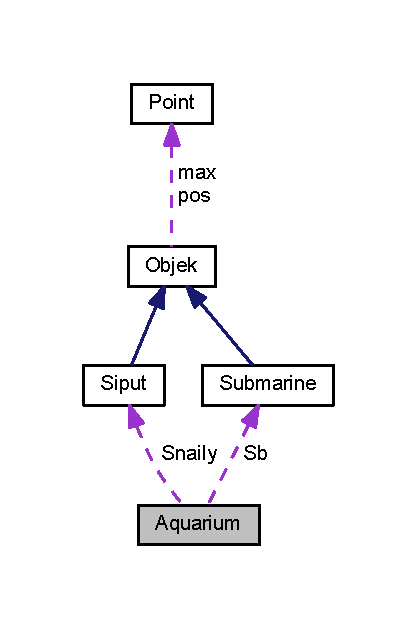
\includegraphics[width=200pt]{class_aquarium__coll__graph}
\end{center}
\end{figure}
\subsection*{Public Member Functions}
\begin{DoxyCompactItemize}
\item 
\mbox{\Hypertarget{class_aquarium_a3cff2b1a50a561f4f231145d44282bcc}\label{class_aquarium_a3cff2b1a50a561f4f231145d44282bcc}} 
{\bfseries Aquarium} (int a, int b)
\item 
\mbox{\Hypertarget{class_aquarium_a7d855672531a2da9655bf42fbd3d3dcc}\label{class_aquarium_a7d855672531a2da9655bf42fbd3d3dcc}} 
int {\bfseries get\+Egg\+State} ()
\item 
\mbox{\Hypertarget{class_aquarium_ac48b93474730e4ebbb69207e8e875760}\label{class_aquarium_ac48b93474730e4ebbb69207e8e875760}} 
void {\bfseries increase\+Egg\+State} ()
\item 
\mbox{\Hypertarget{class_aquarium_ac030a82bcd46ea6b8d7abcb6acfb0481}\label{class_aquarium_ac030a82bcd46ea6b8d7abcb6acfb0481}} 
int {\bfseries get\+Curr\+Egg\+Price} ()
\item 
\mbox{\Hypertarget{class_aquarium_a000a4fa85f8fde473e2df1b6639da9f5}\label{class_aquarium_a000a4fa85f8fde473e2df1b6639da9f5}} 
int {\bfseries get\+Curr\+Food\+Price} ()
\item 
\mbox{\Hypertarget{class_aquarium_ada38a4e23a562f578e99dcbfd29ccc9d}\label{class_aquarium_ada38a4e23a562f578e99dcbfd29ccc9d}} 
int {\bfseries get\+Food\+Up\+Price} ()
\item 
\mbox{\Hypertarget{class_aquarium_ad13cadde72f6ba660ce6807690d6ee67}\label{class_aquarium_ad13cadde72f6ba660ce6807690d6ee67}} 
void {\bfseries upgrade\+Food} ()
\end{DoxyCompactItemize}
\subsection*{Public Attributes}
\begin{DoxyCompactItemize}
\item 
\mbox{\Hypertarget{class_aquarium_aba49eb1d68ec99219e851c9241cdf361}\label{class_aquarium_aba49eb1d68ec99219e851c9241cdf361}} 
\mbox{\hyperlink{class_siput}{Siput}} {\bfseries Snaily}
\item 
\mbox{\Hypertarget{class_aquarium_a8ff32a3dd96479a8095fd7103840cec2}\label{class_aquarium_a8ff32a3dd96479a8095fd7103840cec2}} 
\mbox{\hyperlink{class_submarine}{Submarine}} {\bfseries Sb}
\end{DoxyCompactItemize}
\subsection*{Protected Attributes}
\begin{DoxyCompactItemize}
\item 
\mbox{\Hypertarget{class_aquarium_af20d348c2f202d514383820440df7e1c}\label{class_aquarium_af20d348c2f202d514383820440df7e1c}} 
int {\bfseries egg\+State}
\end{DoxyCompactItemize}
\subsection*{Static Protected Attributes}
\begin{DoxyCompactItemize}
\item 
\mbox{\Hypertarget{class_aquarium_a20ac94b3e0d1dbfa683751599900b68f}\label{class_aquarium_a20ac94b3e0d1dbfa683751599900b68f}} 
static const int {\bfseries food\+Up\+Price} \mbox{[}$\,$\mbox{]} = \{0,300,400,500\}
\item 
\mbox{\Hypertarget{class_aquarium_aeddefcb3757ab680306a3dc12765f791}\label{class_aquarium_aeddefcb3757ab680306a3dc12765f791}} 
static const int {\bfseries egg\+Price} \mbox{[}$\,$\mbox{]} = \{0,2000,3000,4000\}
\item 
\mbox{\Hypertarget{class_aquarium_a0c66fead918aa90dbe07d7e5a110d408}\label{class_aquarium_a0c66fead918aa90dbe07d7e5a110d408}} 
static const int {\bfseries food\+Price} \mbox{[}$\,$\mbox{]} = \{0,15,10,5\}
\end{DoxyCompactItemize}


The documentation for this class was generated from the following file\+:\begin{DoxyCompactItemize}
\item 
C\+:/\+Users/\+Asus/\+Documents/\+O\+O\+P/\+New folder/arkavquarium/\+Arkav\+Quarium/arkavquarium/\+Arkav\+Quarium/Aquarium.\+hpp\end{DoxyCompactItemize}

\hypertarget{class_coin}{}\section{Coin Class Reference}
\label{class_coin}\index{Coin@{Coin}}


Inheritance diagram for Coin\+:\nopagebreak
\begin{figure}[H]
\begin{center}
\leavevmode
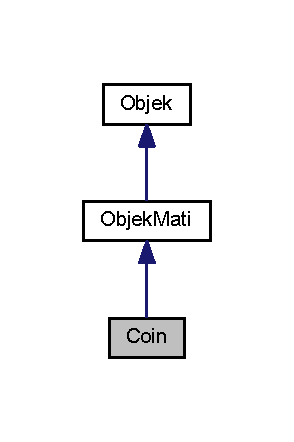
\includegraphics[width=141pt]{class_coin__inherit__graph}
\end{center}
\end{figure}


Collaboration diagram for Coin\+:\nopagebreak
\begin{figure}[H]
\begin{center}
\leavevmode
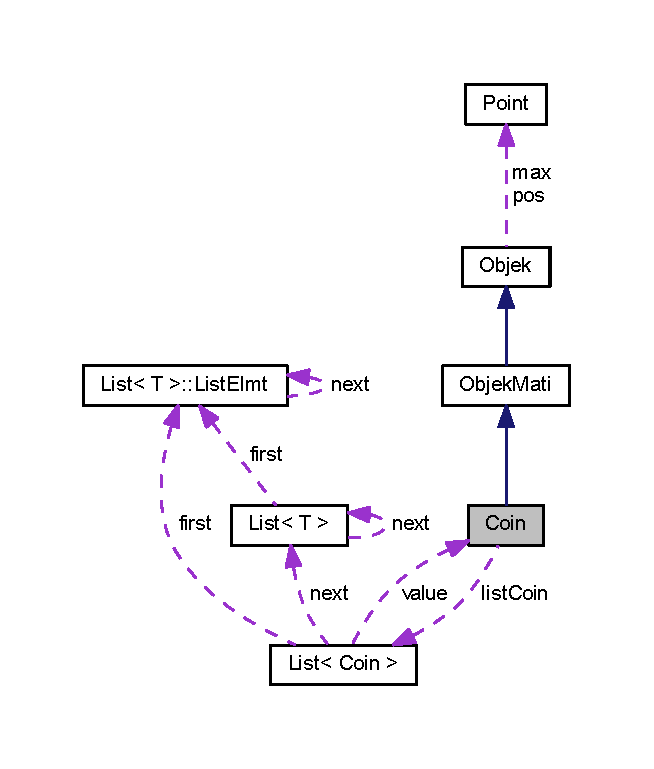
\includegraphics[width=314pt]{class_coin__coll__graph}
\end{center}
\end{figure}
\subsection*{Public Member Functions}
\begin{DoxyCompactItemize}
\item 
\mbox{\Hypertarget{class_coin_a09a841eb6b3edf5f4e6143589825077a}\label{class_coin_a09a841eb6b3edf5f4e6143589825077a}} 
{\bfseries Coin} (int val, int t)
\item 
\mbox{\Hypertarget{class_coin_a3b37ac5e6fe38e884431bc5bafc519fd}\label{class_coin_a3b37ac5e6fe38e884431bc5bafc519fd}} 
{\bfseries Coin} (int val, \mbox{\hyperlink{class_point}{Point}} P, int t)
\item 
\mbox{\Hypertarget{class_coin_ad553fc0811dc55965a1ed96c7060ed6e}\label{class_coin_ad553fc0811dc55965a1ed96c7060ed6e}} 
void {\bfseries remove\+From\+List} ()
\item 
\mbox{\Hypertarget{class_coin_a1e51e734f8cbd7366e4376d9e3439d9e}\label{class_coin_a1e51e734f8cbd7366e4376d9e3439d9e}} 
int {\bfseries get\+Value} ()
\item 
\mbox{\Hypertarget{class_coin_a7bb558fbb0733956d48fe5c6f6758da9}\label{class_coin_a7bb558fbb0733956d48fe5c6f6758da9}} 
void {\bfseries set\+Value} (int v)
\item 
\mbox{\Hypertarget{class_coin_af813e93a2db204d94f981c6151bf6f68}\label{class_coin_af813e93a2db204d94f981c6151bf6f68}} 
void {\bfseries drown} ()
\item 
\mbox{\Hypertarget{class_coin_a623a688d85c3ee9c9d7120eb6f7ea364}\label{class_coin_a623a688d85c3ee9c9d7120eb6f7ea364}} 
void {\bfseries add\+Collected\+Coins} ()
\item 
\mbox{\Hypertarget{class_coin_aac20a35bafe3f05037d32c579e264da2}\label{class_coin_aac20a35bafe3f05037d32c579e264da2}} 
void {\bfseries draw} ()
\end{DoxyCompactItemize}
\subsection*{Static Public Member Functions}
\begin{DoxyCompactItemize}
\item 
\mbox{\Hypertarget{class_coin_a36b1c0683e99eb449e9fbd63aff3a8ee}\label{class_coin_a36b1c0683e99eb449e9fbd63aff3a8ee}} 
static \mbox{\hyperlink{class_list}{List}}$<$ \mbox{\hyperlink{class_coin}{Coin}} $>$ {\bfseries get\+Active\+Coins} ()
\item 
\mbox{\Hypertarget{class_coin_abbf4146f1d9f3356f76a9144c8af5767}\label{class_coin_abbf4146f1d9f3356f76a9144c8af5767}} 
static int {\bfseries get\+Collected\+Coins} ()
\item 
\mbox{\Hypertarget{class_coin_a5fed02f0075539657f2bf3ab65ca062f}\label{class_coin_a5fed02f0075539657f2bf3ab65ca062f}} 
static void {\bfseries dec\+Collected\+Coin} (int val)
\end{DoxyCompactItemize}
\subsection*{Protected Attributes}
\begin{DoxyCompactItemize}
\item 
\mbox{\Hypertarget{class_coin_a3273e38e55be31a1c123fc0a46820467}\label{class_coin_a3273e38e55be31a1c123fc0a46820467}} 
int {\bfseries value}
\item 
\mbox{\Hypertarget{class_coin_add139e05dcc9a7c9447a64a8c359df0b}\label{class_coin_add139e05dcc9a7c9447a64a8c359df0b}} 
int {\bfseries ground\+Timer}
\item 
\mbox{\Hypertarget{class_coin_adf27a764ac814ecd81cc43a6514b3ea1}\label{class_coin_adf27a764ac814ecd81cc43a6514b3ea1}} 
int {\bfseries cointype}
\end{DoxyCompactItemize}
\subsection*{Static Protected Attributes}
\begin{DoxyCompactItemize}
\item 
\mbox{\Hypertarget{class_coin_a453588a8bec6761c106b80c2455d2b8f}\label{class_coin_a453588a8bec6761c106b80c2455d2b8f}} 
static \mbox{\hyperlink{class_list}{List}}$<$ \mbox{\hyperlink{class_coin}{Coin}} $>$ {\bfseries list\+Coin} = \mbox{\hyperlink{class_list}{List}}$<$\mbox{\hyperlink{class_coin}{Coin}}$>$()
\item 
\mbox{\Hypertarget{class_coin_a25fe8e8e24c94da1dd64d50be9703c9f}\label{class_coin_a25fe8e8e24c94da1dd64d50be9703c9f}} 
static int {\bfseries Collected\+Coin} = 0
\end{DoxyCompactItemize}


The documentation for this class was generated from the following file\+:\begin{DoxyCompactItemize}
\item 
C\+:/\+Users/\+Asus/\+Documents/\+O\+O\+P/\+New folder/arkavquarium/\+Arkav\+Quarium/arkavquarium/\+Arkav\+Quarium/Coin.\+hpp\end{DoxyCompactItemize}

\hypertarget{class_fish_food}{}\section{Fish\+Food Class Reference}
\label{class_fish_food}\index{Fish\+Food@{Fish\+Food}}


Inheritance diagram for Fish\+Food\+:\nopagebreak
\begin{figure}[H]
\begin{center}
\leavevmode
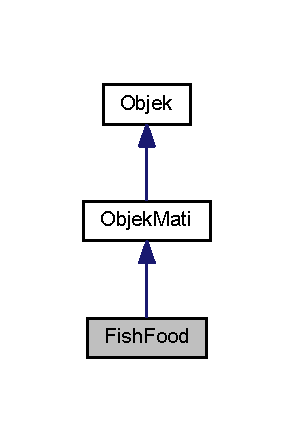
\includegraphics[width=141pt]{class_fish_food__inherit__graph}
\end{center}
\end{figure}


Collaboration diagram for Fish\+Food\+:\nopagebreak
\begin{figure}[H]
\begin{center}
\leavevmode
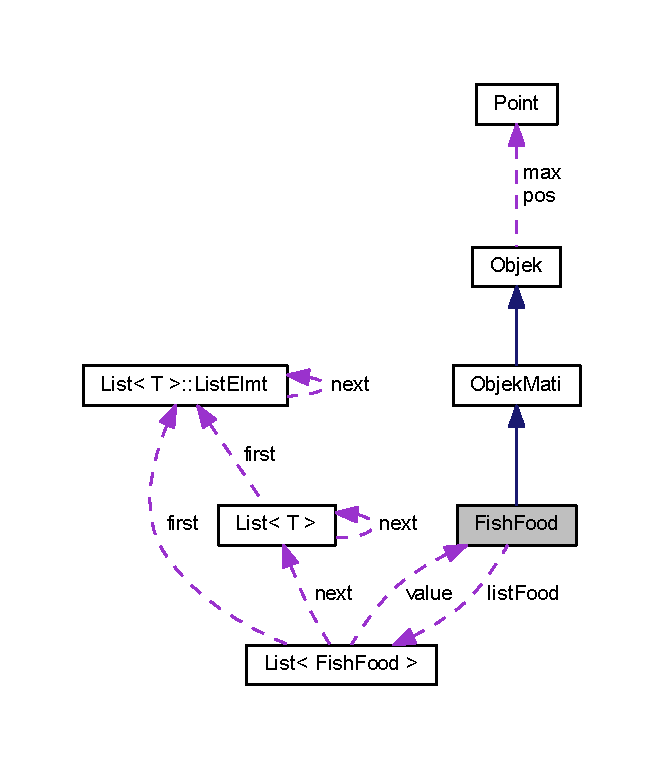
\includegraphics[width=319pt]{class_fish_food__coll__graph}
\end{center}
\end{figure}
\subsection*{Public Member Functions}
\begin{DoxyCompactItemize}
\item 
\mbox{\Hypertarget{class_fish_food_a3e8f3c93069e4c6163dbebca2f424adc}\label{class_fish_food_a3e8f3c93069e4c6163dbebca2f424adc}} 
{\bfseries Fish\+Food} (\mbox{\hyperlink{class_point}{Point}} p)
\item 
\mbox{\Hypertarget{class_fish_food_ab9d6c0fc07ed3ceb8fe31fbfee793bb3}\label{class_fish_food_ab9d6c0fc07ed3ceb8fe31fbfee793bb3}} 
void {\bfseries remove\+From\+List} ()
\item 
\mbox{\Hypertarget{class_fish_food_ac17f2587b9690da0d515cfa91dea6f5a}\label{class_fish_food_ac17f2587b9690da0d515cfa91dea6f5a}} 
void {\bfseries draw} ()
\item 
\mbox{\Hypertarget{class_fish_food_a5cdba669dec2af75a0887801f907cc2d}\label{class_fish_food_a5cdba669dec2af75a0887801f907cc2d}} 
void {\bfseries drown} ()
\end{DoxyCompactItemize}
\subsection*{Static Public Member Functions}
\begin{DoxyCompactItemize}
\item 
\mbox{\Hypertarget{class_fish_food_a68c2d09a1c230c6923c2fe61a50a877e}\label{class_fish_food_a68c2d09a1c230c6923c2fe61a50a877e}} 
static void {\bfseries set\+Food\+Lvl} (int m)
\item 
\mbox{\Hypertarget{class_fish_food_a20b3d2c4fe40c1999cbd1a1339808fb3}\label{class_fish_food_a20b3d2c4fe40c1999cbd1a1339808fb3}} 
static int {\bfseries get\+Food\+Lvl} ()
\item 
\mbox{\Hypertarget{class_fish_food_ab0d24aa0e13cd6a2b5446e223ac09774}\label{class_fish_food_ab0d24aa0e13cd6a2b5446e223ac09774}} 
static void {\bfseries inc\+Food\+Lvl} ()
\item 
\mbox{\Hypertarget{class_fish_food_aa322ac4cedaa7dff4c2a14918bf23948}\label{class_fish_food_aa322ac4cedaa7dff4c2a14918bf23948}} 
static \mbox{\hyperlink{class_list}{List}}$<$ \mbox{\hyperlink{class_fish_food}{Fish\+Food}} $>$ {\bfseries get\+Food\+List} ()
\end{DoxyCompactItemize}
\subsection*{Static Protected Attributes}
\begin{DoxyCompactItemize}
\item 
\mbox{\Hypertarget{class_fish_food_afa5ef582d9cf34bab9d4531366c1f452}\label{class_fish_food_afa5ef582d9cf34bab9d4531366c1f452}} 
static \mbox{\hyperlink{class_list}{List}}$<$ \mbox{\hyperlink{class_fish_food}{Fish\+Food}} $>$ {\bfseries list\+Food} = \mbox{\hyperlink{class_list}{List}}$<$\mbox{\hyperlink{class_fish_food}{Fish\+Food}}$>$()
\item 
\mbox{\Hypertarget{class_fish_food_ac0964c175b990b8a2c2ef14c0fe4afee}\label{class_fish_food_ac0964c175b990b8a2c2ef14c0fe4afee}} 
static int {\bfseries foodlvl} = 1
\end{DoxyCompactItemize}
\subsection*{Additional Inherited Members}


The documentation for this class was generated from the following file\+:\begin{DoxyCompactItemize}
\item 
C\+:/\+Users/\+Asus/\+Documents/\+O\+O\+P/\+New folder/arkavquarium/\+Arkav\+Quarium/arkavquarium/\+Arkav\+Quarium/Fish\+Food.\+hpp\end{DoxyCompactItemize}

\hypertarget{class_guppy}{}\section{Guppy Class Reference}
\label{class_guppy}\index{Guppy@{Guppy}}


Inheritance diagram for Guppy\+:\nopagebreak
\begin{figure}[H]
\begin{center}
\leavevmode
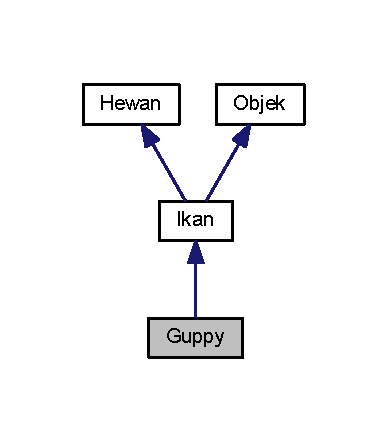
\includegraphics[width=186pt]{class_guppy__inherit__graph}
\end{center}
\end{figure}


Collaboration diagram for Guppy\+:\nopagebreak
\begin{figure}[H]
\begin{center}
\leavevmode
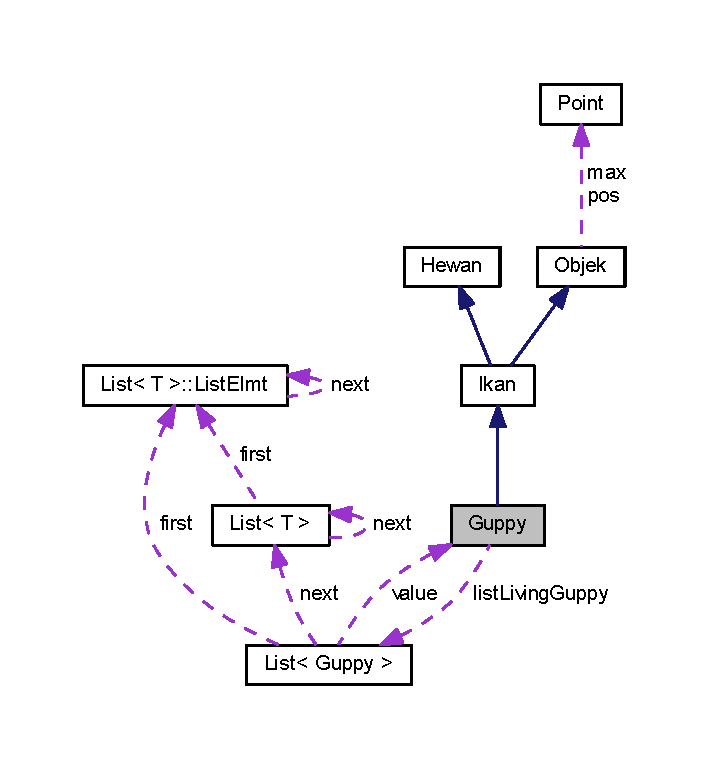
\includegraphics[width=341pt]{class_guppy__coll__graph}
\end{center}
\end{figure}
\subsection*{Public Member Functions}
\begin{DoxyCompactItemize}
\item 
\mbox{\Hypertarget{class_guppy_ae06e1cd99ed7465d2a0b7754153971cd}\label{class_guppy_ae06e1cd99ed7465d2a0b7754153971cd}} 
{\bfseries Guppy} (\mbox{\hyperlink{class_point}{Point}} npos, int n\+Level=1, char c=\textquotesingle{}R\textquotesingle{}, int fooe=0)
\item 
\mbox{\Hypertarget{class_guppy_a4b9e9891d373378b04f953eb7e174703}\label{class_guppy_a4b9e9891d373378b04f953eb7e174703}} 
void {\bfseries decrease\+Health} ()
\item 
\mbox{\Hypertarget{class_guppy_a2fc22c1ccc32961cdfd37522ad05a341}\label{class_guppy_a2fc22c1ccc32961cdfd37522ad05a341}} 
void {\bfseries remove\+From\+List} ()
\item 
\mbox{\Hypertarget{class_guppy_aabf3fb7f79f5d95d25c03ae098f748c1}\label{class_guppy_aabf3fb7f79f5d95d25c03ae098f748c1}} 
\mbox{\hyperlink{class_fish_food}{Fish\+Food}} {\bfseries search\+Makanan} ()
\item 
\mbox{\Hypertarget{class_guppy_a55934fc9069ad5794994785bdba20ba5}\label{class_guppy_a55934fc9069ad5794994785bdba20ba5}} 
void {\bfseries normal\+Move} (int dir\+Deg=0)
\item 
\mbox{\Hypertarget{class_guppy_ae5747e277690dda160686e41822d0967}\label{class_guppy_ae5747e277690dda160686e41822d0967}} 
void {\bfseries move} (int dir\+Deg=0)
\item 
\mbox{\Hypertarget{class_guppy_ad9be268a40b05d84b9394610254179ca}\label{class_guppy_ad9be268a40b05d84b9394610254179ca}} 
void {\bfseries makan} (\mbox{\hyperlink{class_fish_food}{Fish\+Food}} food)
\item 
\mbox{\Hypertarget{class_guppy_a6d6b058e700fe8f7592afe59cd91eada}\label{class_guppy_a6d6b058e700fe8f7592afe59cd91eada}} 
void {\bfseries produce\+Coin} (int price)
\item 
\mbox{\Hypertarget{class_guppy_a3438f0c503f0260034115ace01264cdc}\label{class_guppy_a3438f0c503f0260034115ace01264cdc}} 
void {\bfseries draw} ()
\end{DoxyCompactItemize}
\subsection*{Static Public Member Functions}
\begin{DoxyCompactItemize}
\item 
\mbox{\Hypertarget{class_guppy_a21918ee02e231b7fa97546765d57c1b1}\label{class_guppy_a21918ee02e231b7fa97546765d57c1b1}} 
static \mbox{\hyperlink{class_list}{List}}$<$ \mbox{\hyperlink{class_guppy}{Guppy}} $>$ {\bfseries get\+Guppy\+List} ()
\item 
\mbox{\Hypertarget{class_guppy_a221be82f9bf137d155ca8daccdf3fa41}\label{class_guppy_a221be82f9bf137d155ca8daccdf3fa41}} 
static void {\bfseries draw\+All} ()
\end{DoxyCompactItemize}
\subsection*{Protected Attributes}
\begin{DoxyCompactItemize}
\item 
\mbox{\Hypertarget{class_guppy_ac91b6d5ced32faecdfe47909cb3238c8}\label{class_guppy_ac91b6d5ced32faecdfe47909cb3238c8}} 
int {\bfseries gold\+Timer}
\end{DoxyCompactItemize}
\subsection*{Static Protected Attributes}
\begin{DoxyCompactItemize}
\item 
\mbox{\Hypertarget{class_guppy_a52f825cc6cf31e682a3a3ce27b3f1390}\label{class_guppy_a52f825cc6cf31e682a3a3ce27b3f1390}} 
static \mbox{\hyperlink{class_list}{List}}$<$ \mbox{\hyperlink{class_guppy}{Guppy}} $>$ {\bfseries list\+Living\+Guppy} = \mbox{\hyperlink{class_list}{List}}$<$\mbox{\hyperlink{class_guppy}{Guppy}}$>$()
\item 
\mbox{\Hypertarget{class_guppy_ae474e8947cad2d165e3b80bb6eb6b51f}\label{class_guppy_ae474e8947cad2d165e3b80bb6eb6b51f}} 
static const double {\bfseries speed} = 0.\+5
\end{DoxyCompactItemize}


The documentation for this class was generated from the following file\+:\begin{DoxyCompactItemize}
\item 
C\+:/\+Users/\+Asus/\+Documents/\+O\+O\+P/\+New folder/arkavquarium/\+Arkav\+Quarium/arkavquarium/\+Arkav\+Quarium/Guppy.\+hpp\end{DoxyCompactItemize}

\hypertarget{class_hewan}{}\section{Hewan Class Reference}
\label{class_hewan}\index{Hewan@{Hewan}}


Inheritance diagram for Hewan\+:\nopagebreak
\begin{figure}[H]
\begin{center}
\leavevmode
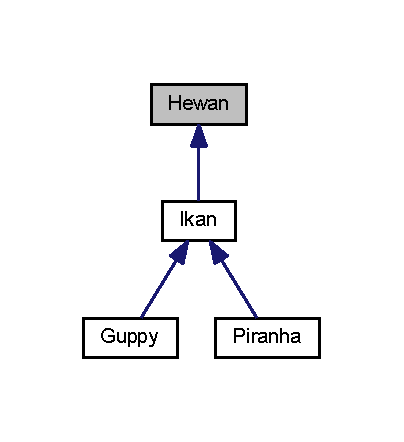
\includegraphics[width=194pt]{class_hewan__inherit__graph}
\end{center}
\end{figure}
\subsection*{Public Member Functions}
\begin{DoxyCompactItemize}
\item 
\mbox{\Hypertarget{class_hewan_a5eee39533ecc3e62eb0c1446909679a7}\label{class_hewan_a5eee39533ecc3e62eb0c1446909679a7}} 
virtual void {\bfseries move} (int)=0
\item 
\mbox{\Hypertarget{class_hewan_a41bb691cef05f54097c61a63e1e32550}\label{class_hewan_a41bb691cef05f54097c61a63e1e32550}} 
virtual void {\bfseries turn} (char)=0
\end{DoxyCompactItemize}


The documentation for this class was generated from the following file\+:\begin{DoxyCompactItemize}
\item 
C\+:/\+Users/\+Asus/\+Documents/\+O\+O\+P/\+New folder/arkavquarium/\+Arkav\+Quarium/arkavquarium/\+Arkav\+Quarium/Hewan.\+hpp\end{DoxyCompactItemize}

\hypertarget{class_ikan}{}\section{Ikan Class Reference}
\label{class_ikan}\index{Ikan@{Ikan}}


Inheritance diagram for Ikan\+:\nopagebreak
\begin{figure}[H]
\begin{center}
\leavevmode
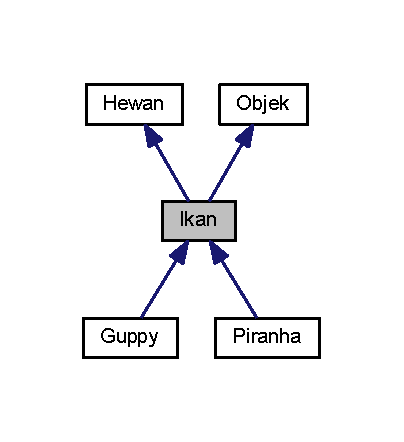
\includegraphics[width=194pt]{class_ikan__inherit__graph}
\end{center}
\end{figure}


Collaboration diagram for Ikan\+:\nopagebreak
\begin{figure}[H]
\begin{center}
\leavevmode
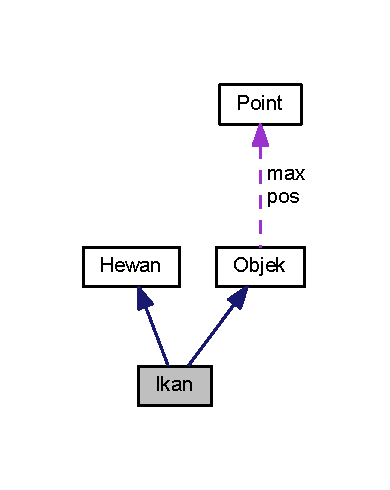
\includegraphics[width=187pt]{class_ikan__coll__graph}
\end{center}
\end{figure}
\subsection*{Public Member Functions}
\begin{DoxyCompactItemize}
\item 
\mbox{\Hypertarget{class_ikan_ad11c2d630dff6f3d9a1129029655f2b4}\label{class_ikan_ad11c2d630dff6f3d9a1129029655f2b4}} 
{\bfseries Ikan} (int nlevel, \mbox{\hyperlink{class_point}{Point}} npos, char c, int fooe)
\item 
\mbox{\Hypertarget{class_ikan_a69070048af8a005276c98a8cd6755edd}\label{class_ikan_a69070048af8a005276c98a8cd6755edd}} 
void {\bfseries turn} (char dir)
\item 
\mbox{\Hypertarget{class_ikan_a58a414cb234c8ce3dfca59831baaa7a9}\label{class_ikan_a58a414cb234c8ce3dfca59831baaa7a9}} 
virtual int {\bfseries get\+Price} ()
\item 
\mbox{\Hypertarget{class_ikan_ae8e8d10470b73a766aa103469a4c9ab6}\label{class_ikan_ae8e8d10470b73a766aa103469a4c9ab6}} 
int {\bfseries get\+Level} ()
\item 
\mbox{\Hypertarget{class_ikan_a03979ad7be7753ac795360fda22b6c9f}\label{class_ikan_a03979ad7be7753ac795360fda22b6c9f}} 
int {\bfseries get\+Health} ()
\item 
\mbox{\Hypertarget{class_ikan_a2059bbceb47a3a2e25013f68aa657f14}\label{class_ikan_a2059bbceb47a3a2e25013f68aa657f14}} 
bool {\bfseries get\+Arah} ()
\item 
\mbox{\Hypertarget{class_ikan_a6018ad3686c28f158e345fa8a8cc96fd}\label{class_ikan_a6018ad3686c28f158e345fa8a8cc96fd}} 
int {\bfseries get\+Food\+Required} ()
\item 
\mbox{\Hypertarget{class_ikan_ac10bd9b8648a4ba070f91a7048b91094}\label{class_ikan_ac10bd9b8648a4ba070f91a7048b91094}} 
int {\bfseries get\+Food\+Eaten} ()
\item 
\mbox{\Hypertarget{class_ikan_abb156038baed8a17815dcab87cc9d93e}\label{class_ikan_abb156038baed8a17815dcab87cc9d93e}} 
int {\bfseries get\+Hunger\+Health} ()
\item 
\mbox{\Hypertarget{class_ikan_ac39d66a7e5548dfa1798566165671d91}\label{class_ikan_ac39d66a7e5548dfa1798566165671d91}} 
virtual int {\bfseries get\+Max\+Health} ()
\item 
\mbox{\Hypertarget{class_ikan_a4ac1a7389722b0d90cdea084eeae0a96}\label{class_ikan_a4ac1a7389722b0d90cdea084eeae0a96}} 
void {\bfseries set\+Level} (int l)
\item 
\mbox{\Hypertarget{class_ikan_ab6ebf8765c816c2fcad976dea7a28fa1}\label{class_ikan_ab6ebf8765c816c2fcad976dea7a28fa1}} 
void {\bfseries set\+Health} (int h)
\item 
\mbox{\Hypertarget{class_ikan_a468c1517b1d7227435f19d495f8b577b}\label{class_ikan_a468c1517b1d7227435f19d495f8b577b}} 
void {\bfseries set\+Arah} ()
\item 
\mbox{\Hypertarget{class_ikan_a38f23cfe05849034843fa1fd6b58fba6}\label{class_ikan_a38f23cfe05849034843fa1fd6b58fba6}} 
void {\bfseries set\+Food\+Eaten} (int s)
\item 
\mbox{\Hypertarget{class_ikan_ad16ad4b60764965c62fb5d2d811aed76}\label{class_ikan_ad16ad4b60764965c62fb5d2d811aed76}} 
void {\bfseries level\+Up} ()
\item 
\mbox{\Hypertarget{class_ikan_a1873e2aadc60b4553c3c1b00fcdc6809}\label{class_ikan_a1873e2aadc60b4553c3c1b00fcdc6809}} 
virtual void {\bfseries produce\+Coin} (int price)=0
\end{DoxyCompactItemize}
\subsection*{Static Public Member Functions}
\begin{DoxyCompactItemize}
\item 
\mbox{\Hypertarget{class_ikan_a4116d64d65c8d7d2eb2cd9bce146d8a1}\label{class_ikan_a4116d64d65c8d7d2eb2cd9bce146d8a1}} 
static int {\bfseries get\+Default\+Price} ()
\end{DoxyCompactItemize}
\subsection*{Protected Attributes}
\begin{DoxyCompactItemize}
\item 
\mbox{\Hypertarget{class_ikan_a1c10f6164f3d953e4a269f14206dd77e}\label{class_ikan_a1c10f6164f3d953e4a269f14206dd77e}} 
int {\bfseries health}
\item 
\mbox{\Hypertarget{class_ikan_ab9615db3b2a13cb2ac7f443137eec7db}\label{class_ikan_ab9615db3b2a13cb2ac7f443137eec7db}} 
int {\bfseries level}
\item 
\mbox{\Hypertarget{class_ikan_ae0eec1e48cd85ed1c8cdefc08d58b008}\label{class_ikan_ae0eec1e48cd85ed1c8cdefc08d58b008}} 
bool {\bfseries hunger\+Stat}
\item 
\mbox{\Hypertarget{class_ikan_a0c14a4fe8f03401597701dd35e939615}\label{class_ikan_a0c14a4fe8f03401597701dd35e939615}} 
bool {\bfseries arah}
\item 
\mbox{\Hypertarget{class_ikan_a9173ea1ea901676851ee27e7a493a975}\label{class_ikan_a9173ea1ea901676851ee27e7a493a975}} 
int {\bfseries food\+Eaten}
\item 
\mbox{\Hypertarget{class_ikan_aef505e7bd95177f9aa47e622b607615f}\label{class_ikan_aef505e7bd95177f9aa47e622b607615f}} 
char {\bfseries state\+DirH}
\item 
\mbox{\Hypertarget{class_ikan_af5f0010ebce279593e6eb10c9e40a302}\label{class_ikan_af5f0010ebce279593e6eb10c9e40a302}} 
char {\bfseries state\+DirV}
\item 
\mbox{\Hypertarget{class_ikan_a52e4eb9fc490ebc0e127a8ec6c702225}\label{class_ikan_a52e4eb9fc490ebc0e127a8ec6c702225}} 
float {\bfseries dir\+Degree}
\end{DoxyCompactItemize}
\subsection*{Static Protected Attributes}
\begin{DoxyCompactItemize}
\item 
\mbox{\Hypertarget{class_ikan_a603c4e378dd174f68c0d92fd6abc6c8c}\label{class_ikan_a603c4e378dd174f68c0d92fd6abc6c8c}} 
static int const {\bfseries price} \mbox{[}$\,$\mbox{]} = \{0,100,200,300\}
\item 
\mbox{\Hypertarget{class_ikan_a6abbf38f589105f5175268d2dfca3026}\label{class_ikan_a6abbf38f589105f5175268d2dfca3026}} 
static int const {\bfseries max\+Health} \mbox{[}$\,$\mbox{]} = \{0,3000,3500,4500\}
\item 
\mbox{\Hypertarget{class_ikan_a3bfba959e11072b42cf5e966489dcf6c}\label{class_ikan_a3bfba959e11072b42cf5e966489dcf6c}} 
static int const {\bfseries food\+Required} \mbox{[}$\,$\mbox{]} = \{0,5,10,10000\}
\item 
\mbox{\Hypertarget{class_ikan_a6316ec85d20b95b798753e2b36da9ae8}\label{class_ikan_a6316ec85d20b95b798753e2b36da9ae8}} 
static float const {\bfseries hunger\+Percent} = 0.\+4
\end{DoxyCompactItemize}


The documentation for this class was generated from the following file\+:\begin{DoxyCompactItemize}
\item 
C\+:/\+Users/\+Asus/\+Documents/\+O\+O\+P/\+New folder/arkavquarium/\+Arkav\+Quarium/arkavquarium/\+Arkav\+Quarium/Ikan.\+hpp\end{DoxyCompactItemize}

\hypertarget{class_list}{}\section{List$<$ T $>$ Class Template Reference}
\label{class_list}\index{List$<$ T $>$@{List$<$ T $>$}}


Collaboration diagram for List$<$ T $>$\+:\nopagebreak
\begin{figure}[H]
\begin{center}
\leavevmode
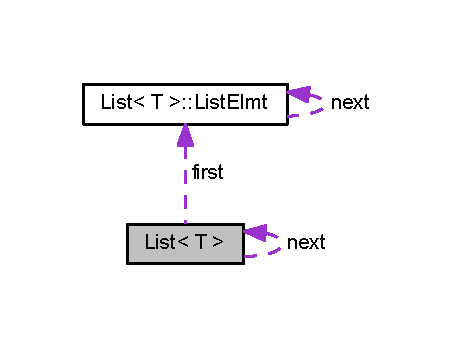
\includegraphics[width=218pt]{class_list__coll__graph}
\end{center}
\end{figure}
\subsection*{Classes}
\begin{DoxyCompactItemize}
\item 
class \mbox{\hyperlink{class_list_1_1_list_elmt}{List\+Elmt}}
\end{DoxyCompactItemize}
\subsection*{Public Member Functions}
\begin{DoxyCompactItemize}
\item 
\mbox{\Hypertarget{class_list_ac657a86ef824f9ec5fea01e15445d231}\label{class_list_ac657a86ef824f9ec5fea01e15445d231}} 
{\bfseries List} (T val)
\item 
\mbox{\Hypertarget{class_list_a73f8b1d313382daffeeeed552f42da2f}\label{class_list_a73f8b1d313382daffeeeed552f42da2f}} 
bool {\bfseries is\+Empty} ()
\item 
\mbox{\Hypertarget{class_list_a70aec33dadb7d317f83f1eb4090cfc51}\label{class_list_a70aec33dadb7d317f83f1eb4090cfc51}} 
{\bfseries List} (const \mbox{\hyperlink{class_list}{List}} \&L)
\item 
\mbox{\Hypertarget{class_list_a560c8d6e0ded475626c67661ee24757e}\label{class_list_a560c8d6e0ded475626c67661ee24757e}} 
T {\bfseries get} (int i)
\item 
\mbox{\Hypertarget{class_list_ab79d41fb024f8315a0bf2730be8b3554}\label{class_list_ab79d41fb024f8315a0bf2730be8b3554}} 
int {\bfseries find} (T val)
\item 
\mbox{\Hypertarget{class_list_a0f4a4d47dc4f9184fe341de6f83031cd}\label{class_list_a0f4a4d47dc4f9184fe341de6f83031cd}} 
bool {\bfseries is\+One\+Elmt} ()
\item 
\mbox{\Hypertarget{class_list_a8dc109bc3840706b2ff77c30a01b1f14}\label{class_list_a8dc109bc3840706b2ff77c30a01b1f14}} 
void {\bfseries add} (T val)
\item 
\mbox{\Hypertarget{class_list_a45978e2ed970993afbf0e5429a5a67d0}\label{class_list_a45978e2ed970993afbf0e5429a5a67d0}} 
void {\bfseries remove} (T val)
\item 
\mbox{\Hypertarget{class_list_a28487cea2818c83adbf1187312340db9}\label{class_list_a28487cea2818c83adbf1187312340db9}} 
T {\bfseries pop\+Last} ()
\item 
\mbox{\Hypertarget{class_list_a87b60ed1c9d849738551043b0368b2df}\label{class_list_a87b60ed1c9d849738551043b0368b2df}} 
\mbox{\hyperlink{class_list}{List}} \& {\bfseries operator$<$$<$} (T val)
\item 
\mbox{\Hypertarget{class_list_adb7eaeb3f3d763702a08f329d0efb574}\label{class_list_adb7eaeb3f3d763702a08f329d0efb574}} 
\mbox{\hyperlink{class_list}{List}} \& {\bfseries operator$>$$>$} (T \&val)
\item 
\mbox{\Hypertarget{class_list_a91bfb3d2b503208f0e163369794fe668}\label{class_list_a91bfb3d2b503208f0e163369794fe668}} 
void {\bfseries draw\+All} ()
\item 
\mbox{\Hypertarget{class_list_ac657a86ef824f9ec5fea01e15445d231}\label{class_list_ac657a86ef824f9ec5fea01e15445d231}} 
{\bfseries List} (T val)
\item 
\mbox{\Hypertarget{class_list_ae23d6cb859d18efa01c7744d4b8b038e}\label{class_list_ae23d6cb859d18efa01c7744d4b8b038e}} 
void {\bfseries clone} (const \mbox{\hyperlink{class_list}{List}}$<$ T $>$ \&L)
\item 
\mbox{\Hypertarget{class_list_a73f8b1d313382daffeeeed552f42da2f}\label{class_list_a73f8b1d313382daffeeeed552f42da2f}} 
bool {\bfseries is\+Empty} ()
\item 
\mbox{\Hypertarget{class_list_a560c8d6e0ded475626c67661ee24757e}\label{class_list_a560c8d6e0ded475626c67661ee24757e}} 
T {\bfseries get} (int i)
\item 
\mbox{\Hypertarget{class_list_ab79d41fb024f8315a0bf2730be8b3554}\label{class_list_ab79d41fb024f8315a0bf2730be8b3554}} 
int {\bfseries find} (T val)
\item 
\mbox{\Hypertarget{class_list_a0f4a4d47dc4f9184fe341de6f83031cd}\label{class_list_a0f4a4d47dc4f9184fe341de6f83031cd}} 
bool {\bfseries is\+One\+Elmt} ()
\item 
\mbox{\Hypertarget{class_list_a8dc109bc3840706b2ff77c30a01b1f14}\label{class_list_a8dc109bc3840706b2ff77c30a01b1f14}} 
void {\bfseries add} (T val)
\item 
\mbox{\Hypertarget{class_list_a45978e2ed970993afbf0e5429a5a67d0}\label{class_list_a45978e2ed970993afbf0e5429a5a67d0}} 
void {\bfseries remove} (T val)
\item 
\mbox{\Hypertarget{class_list_a99c77c6212ed68675ff4559dbd95df85}\label{class_list_a99c77c6212ed68675ff4559dbd95df85}} 
\mbox{\hyperlink{class_list_1_1_list_elmt}{List\+Elmt}} \& {\bfseries operator$<$$<$} (T val)
\item 
\mbox{\Hypertarget{class_list_a70b6f1ffb63381525434254470f9b5d5}\label{class_list_a70b6f1ffb63381525434254470f9b5d5}} 
\mbox{\hyperlink{class_list_1_1_list_elmt}{List\+Elmt}} \& {\bfseries operator$>$$>$} (T val)
\item 
\mbox{\Hypertarget{class_list_a2497bdf42246d61237aaf046c116183a}\label{class_list_a2497bdf42246d61237aaf046c116183a}} 
int {\bfseries size} ()
\item 
\mbox{\Hypertarget{class_list_a91bfb3d2b503208f0e163369794fe668}\label{class_list_a91bfb3d2b503208f0e163369794fe668}} 
void {\bfseries draw\+All} ()
\item 
\mbox{\Hypertarget{class_list_a988389f868a7422d4fbbc557052467ca}\label{class_list_a988389f868a7422d4fbbc557052467ca}} 
void {\bfseries move\+All} ()
\item 
\mbox{\Hypertarget{class_list_add432fe9fbf1676760f25925017b3600}\label{class_list_add432fe9fbf1676760f25925017b3600}} 
void {\bfseries drown\+All} ()
\item 
\mbox{\Hypertarget{class_list_a29ce93b0dcefe3fd759debe9d1749ff4}\label{class_list_a29ce93b0dcefe3fd759debe9d1749ff4}} 
void {\bfseries print\+All} ()
\end{DoxyCompactItemize}
\subsection*{Public Attributes}
\begin{DoxyCompactItemize}
\item 
\mbox{\Hypertarget{class_list_a2bb760765b228099a24741eb8c286bcb}\label{class_list_a2bb760765b228099a24741eb8c286bcb}} 
\mbox{\hyperlink{class_list_1_1_list_elmt}{List\+Elmt}} $\ast$ {\bfseries first}
\end{DoxyCompactItemize}
\subsection*{Protected Attributes}
\begin{DoxyCompactItemize}
\item 
\mbox{\Hypertarget{class_list_a9d5d9c4ec56d10e1f756de27d4e72dd9}\label{class_list_a9d5d9c4ec56d10e1f756de27d4e72dd9}} 
T {\bfseries value}
\item 
\mbox{\Hypertarget{class_list_a8d9eb1ce93f0c564bf7b1099014f9887}\label{class_list_a8d9eb1ce93f0c564bf7b1099014f9887}} 
int {\bfseries num}
\item 
\mbox{\Hypertarget{class_list_a141a9cba941ab2d7a922d90356648fcf}\label{class_list_a141a9cba941ab2d7a922d90356648fcf}} 
\mbox{\hyperlink{class_list}{List}} $\ast$ {\bfseries next}
\end{DoxyCompactItemize}
\subsection*{Friends}
\begin{DoxyCompactItemize}
\item 
\mbox{\Hypertarget{class_list_a4d459cc571f6d70ac4f85ca6eebea471}\label{class_list_a4d459cc571f6d70ac4f85ca6eebea471}} 
ostream \& {\bfseries operator$<$$<$} (ostream \&out, \mbox{\hyperlink{class_list}{List}} \&L)
\item 
\mbox{\Hypertarget{class_list_a0c8949f7ee7e923600d0fe050ea74975}\label{class_list_a0c8949f7ee7e923600d0fe050ea74975}} 
istream \& {\bfseries operator$>$$>$} (istream \&in, \mbox{\hyperlink{class_list}{List}} \&L)
\item 
\mbox{\Hypertarget{class_list_a4d459cc571f6d70ac4f85ca6eebea471}\label{class_list_a4d459cc571f6d70ac4f85ca6eebea471}} 
ostream \& {\bfseries operator$<$$<$} (ostream \&out, \mbox{\hyperlink{class_list}{List}} \&L)
\end{DoxyCompactItemize}


The documentation for this class was generated from the following files\+:\begin{DoxyCompactItemize}
\item 
C\+:/\+Users/\+Asus/\+Documents/\+O\+O\+P/\+New folder/arkavquarium/\+Arkav\+Quarium/arkavquarium/\+Arkav\+Quarium/List.\+cpp\item 
C\+:/\+Users/\+Asus/\+Documents/\+O\+O\+P/\+New folder/arkavquarium/\+Arkav\+Quarium/arkavquarium/\+Arkav\+Quarium/List.\+hpp\end{DoxyCompactItemize}

\hypertarget{class_list_1_1_list_elmt}{}\section{List$<$ T $>$\+:\+:List\+Elmt Class Reference}
\label{class_list_1_1_list_elmt}\index{List$<$ T $>$\+::\+List\+Elmt@{List$<$ T $>$\+::\+List\+Elmt}}


Collaboration diagram for List$<$ T $>$\+:\+:List\+Elmt\+:\nopagebreak
\begin{figure}[H]
\begin{center}
\leavevmode
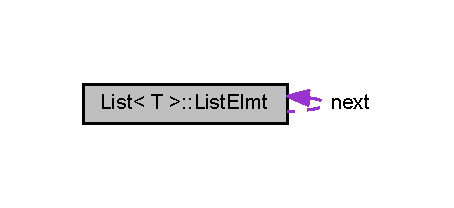
\includegraphics[width=218pt]{class_list_1_1_list_elmt__coll__graph}
\end{center}
\end{figure}
\subsection*{Public Member Functions}
\begin{DoxyCompactItemize}
\item 
\mbox{\Hypertarget{class_list_1_1_list_elmt_ab438c015ce36ca7c14af6adaa6a08d93}\label{class_list_1_1_list_elmt_ab438c015ce36ca7c14af6adaa6a08d93}} 
{\bfseries List\+Elmt} (T val)
\item 
\mbox{\Hypertarget{class_list_1_1_list_elmt_a3097e5bc3f9300c7706cae4f88dbd50b}\label{class_list_1_1_list_elmt_a3097e5bc3f9300c7706cae4f88dbd50b}} 
{\bfseries List\+Elmt} (\mbox{\hyperlink{class_list_1_1_list_elmt}{List\+Elmt}} $\ast$L)
\item 
\mbox{\Hypertarget{class_list_1_1_list_elmt_af00a0092ec26ea7650233c5870b519f8}\label{class_list_1_1_list_elmt_af00a0092ec26ea7650233c5870b519f8}} 
T {\bfseries get} (int i)
\item 
\mbox{\Hypertarget{class_list_1_1_list_elmt_a6df28778d2345a67b1b5c2818b655d1b}\label{class_list_1_1_list_elmt_a6df28778d2345a67b1b5c2818b655d1b}} 
\mbox{\hyperlink{class_list_1_1_list_elmt}{List\+Elmt}} {\bfseries get\+Next} ()
\item 
\mbox{\Hypertarget{class_list_1_1_list_elmt_acdadb7aaa8f64139345af339c0a2d403}\label{class_list_1_1_list_elmt_acdadb7aaa8f64139345af339c0a2d403}} 
int {\bfseries find} (T val)
\item 
\mbox{\Hypertarget{class_list_1_1_list_elmt_a611d9095a4ad03667ae2d4645f4183fa}\label{class_list_1_1_list_elmt_a611d9095a4ad03667ae2d4645f4183fa}} 
void {\bfseries add} (T val)
\item 
\mbox{\Hypertarget{class_list_1_1_list_elmt_a1a5d2c9bf849b19bb10ccbf61191b9fe}\label{class_list_1_1_list_elmt_a1a5d2c9bf849b19bb10ccbf61191b9fe}} 
void {\bfseries remove} (T val)
\item 
\mbox{\Hypertarget{class_list_1_1_list_elmt_a6076563091d1202d4d2a2e2e4343fee6}\label{class_list_1_1_list_elmt_a6076563091d1202d4d2a2e2e4343fee6}} 
void {\bfseries clone} (\mbox{\hyperlink{class_list_1_1_list_elmt}{List\+Elmt}} $\ast$L)
\item 
\mbox{\Hypertarget{class_list_1_1_list_elmt_a189acffdbee3c417833df53767b1d913}\label{class_list_1_1_list_elmt_a189acffdbee3c417833df53767b1d913}} 
T {\bfseries pop\+Last} ()
\item 
\mbox{\Hypertarget{class_list_1_1_list_elmt_a720cdaba23537a0ba23ed4879d74a5eb}\label{class_list_1_1_list_elmt_a720cdaba23537a0ba23ed4879d74a5eb}} 
\mbox{\hyperlink{class_list_1_1_list_elmt}{List\+Elmt}} \& {\bfseries operator$<$$<$} (T val)
\item 
\mbox{\Hypertarget{class_list_1_1_list_elmt_aa4eca3f1464853446749f71f5e4b3a75}\label{class_list_1_1_list_elmt_aa4eca3f1464853446749f71f5e4b3a75}} 
\mbox{\hyperlink{class_list_1_1_list_elmt}{List\+Elmt}} \& {\bfseries operator$>$$>$} (T \&val)
\item 
\mbox{\Hypertarget{class_list_1_1_list_elmt_ae6c3454b32232bc27b4e3887436e0f5a}\label{class_list_1_1_list_elmt_ae6c3454b32232bc27b4e3887436e0f5a}} 
int {\bfseries size} ()
\item 
\mbox{\Hypertarget{class_list_1_1_list_elmt_a55c438b06cd2c6f10d6cbaf4b72f8f7e}\label{class_list_1_1_list_elmt_a55c438b06cd2c6f10d6cbaf4b72f8f7e}} 
void {\bfseries draw\+All} ()
\item 
\mbox{\Hypertarget{class_list_1_1_list_elmt_a99c0d22ad34a738a7864abc39352d53e}\label{class_list_1_1_list_elmt_a99c0d22ad34a738a7864abc39352d53e}} 
void {\bfseries print\+All} ()
\item 
\mbox{\Hypertarget{class_list_1_1_list_elmt_af273cbab167d2664eb32658af35f9139}\label{class_list_1_1_list_elmt_af273cbab167d2664eb32658af35f9139}} 
void {\bfseries move\+All} ()
\item 
\mbox{\Hypertarget{class_list_1_1_list_elmt_af25990e73eacc00fcbdf9b2805fcf1a9}\label{class_list_1_1_list_elmt_af25990e73eacc00fcbdf9b2805fcf1a9}} 
void {\bfseries drown\+All} ()
\end{DoxyCompactItemize}
\subsection*{Public Attributes}
\begin{DoxyCompactItemize}
\item 
\mbox{\Hypertarget{class_list_1_1_list_elmt_a4fef3eaff9c2e20ff9b2212f6f142329}\label{class_list_1_1_list_elmt_a4fef3eaff9c2e20ff9b2212f6f142329}} 
T {\bfseries value}
\item 
\mbox{\Hypertarget{class_list_1_1_list_elmt_a8c4d50e468d7832c816b6fcaef04157d}\label{class_list_1_1_list_elmt_a8c4d50e468d7832c816b6fcaef04157d}} 
\mbox{\hyperlink{class_list_1_1_list_elmt}{List\+Elmt}} $\ast$ {\bfseries next}
\end{DoxyCompactItemize}
\subsection*{Friends}
\begin{DoxyCompactItemize}
\item 
\mbox{\Hypertarget{class_list_1_1_list_elmt_a05cb8dec2afd3ce9e7b792c70b3804dd}\label{class_list_1_1_list_elmt_a05cb8dec2afd3ce9e7b792c70b3804dd}} 
ostream \& {\bfseries operator$<$$<$} (ostream \&out, \mbox{\hyperlink{class_list_1_1_list_elmt}{List\+Elmt}} \&L)
\item 
\mbox{\Hypertarget{class_list_1_1_list_elmt_ac932b9a069cfc0c2e3ca8924e98da68e}\label{class_list_1_1_list_elmt_ac932b9a069cfc0c2e3ca8924e98da68e}} 
istream \& {\bfseries operator$>$$>$} (istream \&in, \mbox{\hyperlink{class_list_1_1_list_elmt}{List\+Elmt}} \&L)
\end{DoxyCompactItemize}


The documentation for this class was generated from the following file\+:\begin{DoxyCompactItemize}
\item 
C\+:/\+Users/\+Asus/\+Documents/\+O\+O\+P/\+New folder/arkavquarium/\+Arkav\+Quarium/arkavquarium/\+Arkav\+Quarium/List.\+hpp\end{DoxyCompactItemize}

\hypertarget{class_objek}{}\section{Objek Class Reference}
\label{class_objek}\index{Objek@{Objek}}


Inheritance diagram for Objek\+:\nopagebreak
\begin{figure}[H]
\begin{center}
\leavevmode
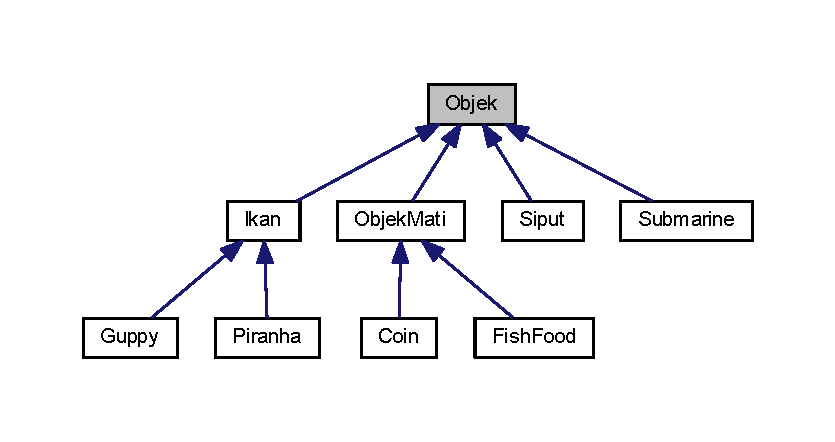
\includegraphics[width=350pt]{class_objek__inherit__graph}
\end{center}
\end{figure}


Collaboration diagram for Objek\+:\nopagebreak
\begin{figure}[H]
\begin{center}
\leavevmode
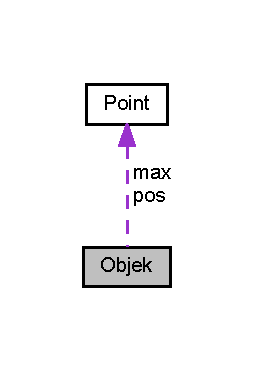
\includegraphics[width=123pt]{class_objek__coll__graph}
\end{center}
\end{figure}
\subsection*{Public Member Functions}
\begin{DoxyCompactItemize}
\item 
\mbox{\Hypertarget{class_objek_a8b3edd96c47dd89f616feccb56390af9}\label{class_objek_a8b3edd96c47dd89f616feccb56390af9}} 
{\bfseries Objek} (\mbox{\hyperlink{class_point}{Point}} P)
\item 
\mbox{\Hypertarget{class_objek_a544b78e0a79f9f99b1ac8271c6fa4972}\label{class_objek_a544b78e0a79f9f99b1ac8271c6fa4972}} 
\mbox{\hyperlink{class_point}{Point}} {\bfseries get\+Point} ()
\item 
\mbox{\Hypertarget{class_objek_ac41425d23ee5fd6d9a74b32470d9ea57}\label{class_objek_ac41425d23ee5fd6d9a74b32470d9ea57}} 
int {\bfseries get\+Id} ()
\item 
\mbox{\Hypertarget{class_objek_a557437419b822a9b535c791b59db5a29}\label{class_objek_a557437419b822a9b535c791b59db5a29}} 
void {\bfseries set\+Point} (\mbox{\hyperlink{class_point}{Point}} P)
\item 
\mbox{\Hypertarget{class_objek_abccef8e9b61b3ccee04c812da69345f9}\label{class_objek_abccef8e9b61b3ccee04c812da69345f9}} 
\mbox{\hyperlink{class_point}{Point}} {\bfseries get\+Batas} ()
\item 
\mbox{\Hypertarget{class_objek_a3e0a75a56419dff5258f4603750bc5f1}\label{class_objek_a3e0a75a56419dff5258f4603750bc5f1}} 
bool {\bfseries operator==} (\mbox{\hyperlink{class_objek}{Objek}} O)
\end{DoxyCompactItemize}
\subsection*{Static Public Member Functions}
\begin{DoxyCompactItemize}
\item 
\mbox{\Hypertarget{class_objek_a4a83ce5b1fb538f6700c7d804b83d428}\label{class_objek_a4a83ce5b1fb538f6700c7d804b83d428}} 
static void {\bfseries initialize\+Max\+Point} (\mbox{\hyperlink{class_point}{Point}} P)
\item 
\mbox{\Hypertarget{class_objek_a2e34d2cd634f680f10b0c72af5764128}\label{class_objek_a2e34d2cd634f680f10b0c72af5764128}} 
static void {\bfseries set\+Max\+Point} (\mbox{\hyperlink{class_point}{Point}} P)
\end{DoxyCompactItemize}
\subsection*{Protected Attributes}
\begin{DoxyCompactItemize}
\item 
\mbox{\Hypertarget{class_objek_aefee1657485871dd407ef4866364b821}\label{class_objek_aefee1657485871dd407ef4866364b821}} 
int {\bfseries id}
\item 
\mbox{\Hypertarget{class_objek_aca6817c5aff91ab98bda2c024a269428}\label{class_objek_aca6817c5aff91ab98bda2c024a269428}} 
\mbox{\hyperlink{class_point}{Point}} {\bfseries pos}
\end{DoxyCompactItemize}
\subsection*{Static Protected Attributes}
\begin{DoxyCompactItemize}
\item 
\mbox{\Hypertarget{class_objek_aeda3bebcf4abfba4d5ff64a03c16dbc6}\label{class_objek_aeda3bebcf4abfba4d5ff64a03c16dbc6}} 
static \mbox{\hyperlink{class_point}{Point}} {\bfseries max} = \mbox{\hyperlink{class_point}{Point}}(500,500)
\item 
\mbox{\Hypertarget{class_objek_aa3eeea111826d0cc0635c7a95d1b6e43}\label{class_objek_aa3eeea111826d0cc0635c7a95d1b6e43}} 
static int {\bfseries id\+List} = 0
\end{DoxyCompactItemize}


The documentation for this class was generated from the following file\+:\begin{DoxyCompactItemize}
\item 
C\+:/\+Users/\+Asus/\+Documents/\+O\+O\+P/\+New folder/arkavquarium/\+Arkav\+Quarium/arkavquarium/\+Arkav\+Quarium/Objek.\+hpp\end{DoxyCompactItemize}

\hypertarget{class_objek_mati}{}\section{Objek\+Mati Class Reference}
\label{class_objek_mati}\index{Objek\+Mati@{Objek\+Mati}}


Inheritance diagram for Objek\+Mati\+:\nopagebreak
\begin{figure}[H]
\begin{center}
\leavevmode
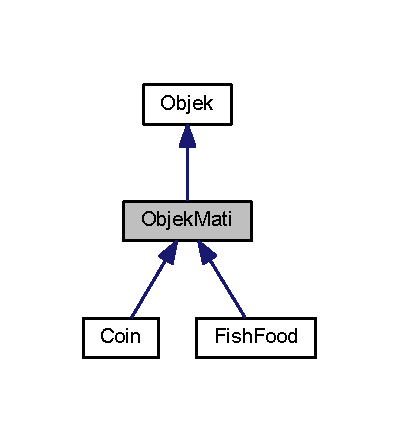
\includegraphics[width=192pt]{class_objek_mati__inherit__graph}
\end{center}
\end{figure}


Collaboration diagram for Objek\+Mati\+:\nopagebreak
\begin{figure}[H]
\begin{center}
\leavevmode
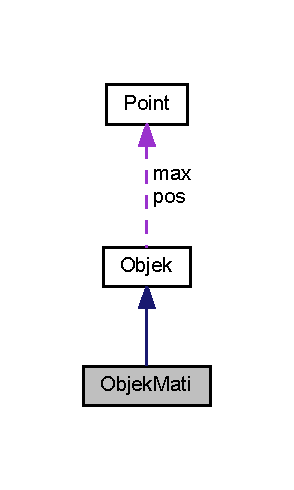
\includegraphics[width=141pt]{class_objek_mati__coll__graph}
\end{center}
\end{figure}
\subsection*{Public Member Functions}
\begin{DoxyCompactItemize}
\item 
\mbox{\Hypertarget{class_objek_mati_a4dc54dc2f5a9c6f3d7a6e692c5dd3b52}\label{class_objek_mati_a4dc54dc2f5a9c6f3d7a6e692c5dd3b52}} 
{\bfseries Objek\+Mati} (\mbox{\hyperlink{class_point}{Point}} P)
\item 
\mbox{\Hypertarget{class_objek_mati_ae95bd4f88da6861ddff7c129cf873f31}\label{class_objek_mati_ae95bd4f88da6861ddff7c129cf873f31}} 
virtual void {\bfseries drown} ()
\end{DoxyCompactItemize}
\subsection*{Static Public Member Functions}
\begin{DoxyCompactItemize}
\item 
\mbox{\Hypertarget{class_objek_mati_aab2918cafc29ccf19de4d40d62002ef4}\label{class_objek_mati_aab2918cafc29ccf19de4d40d62002ef4}} 
static const double {\bfseries get\+Drown\+Speed} ()
\end{DoxyCompactItemize}
\subsection*{Static Protected Attributes}
\begin{DoxyCompactItemize}
\item 
\mbox{\Hypertarget{class_objek_mati_a333ce61c14105232d5ae8d6bc4549f5e}\label{class_objek_mati_a333ce61c14105232d5ae8d6bc4549f5e}} 
static const double {\bfseries speed\+Drown} = 0.\+1
\end{DoxyCompactItemize}
\subsection*{Additional Inherited Members}


The documentation for this class was generated from the following file\+:\begin{DoxyCompactItemize}
\item 
C\+:/\+Users/\+Asus/\+Documents/\+O\+O\+P/\+New folder/arkavquarium/\+Arkav\+Quarium/arkavquarium/\+Arkav\+Quarium/Objek\+Mati.\+hpp\end{DoxyCompactItemize}

\hypertarget{class_piranha}{}\section{Piranha Class Reference}
\label{class_piranha}\index{Piranha@{Piranha}}


Inheritance diagram for Piranha\+:\nopagebreak
\begin{figure}[H]
\begin{center}
\leavevmode
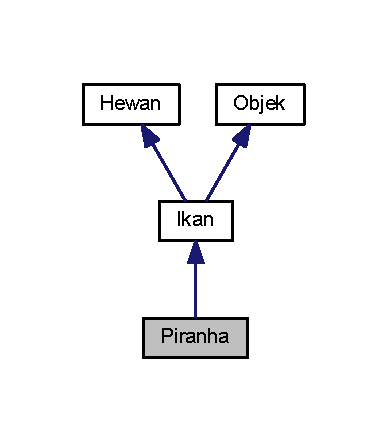
\includegraphics[width=186pt]{class_piranha__inherit__graph}
\end{center}
\end{figure}


Collaboration diagram for Piranha\+:\nopagebreak
\begin{figure}[H]
\begin{center}
\leavevmode
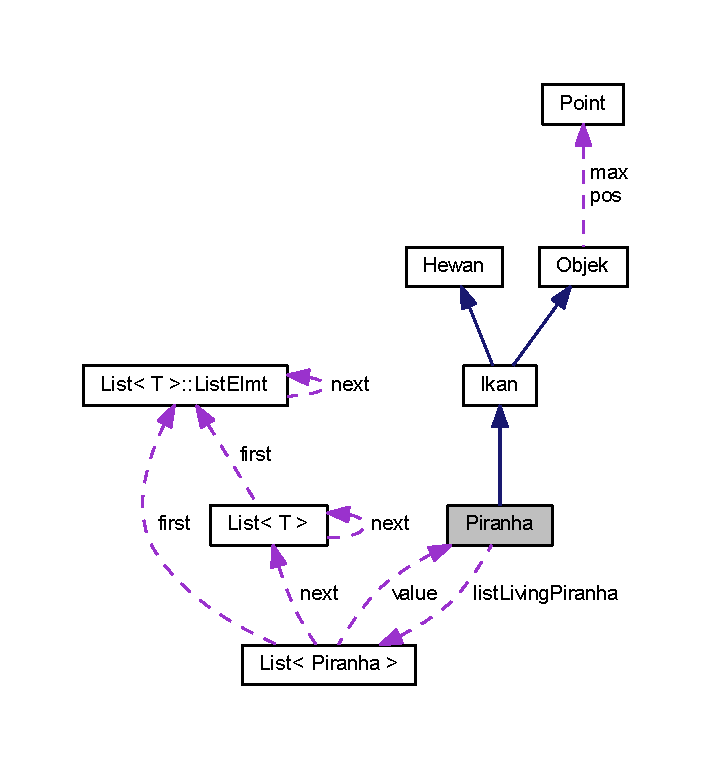
\includegraphics[width=342pt]{class_piranha__coll__graph}
\end{center}
\end{figure}
\subsection*{Public Member Functions}
\begin{DoxyCompactItemize}
\item 
\mbox{\Hypertarget{class_piranha_ac3745db6d47c7621edb8df6fecb72f10}\label{class_piranha_ac3745db6d47c7621edb8df6fecb72f10}} 
{\bfseries Piranha} (\mbox{\hyperlink{class_point}{Point}} npos, int n\+Level=1, char c=\textquotesingle{}R\textquotesingle{}, int fooe=0)
\item 
\mbox{\Hypertarget{class_piranha_a5941759967235fffe0df68de713c6b70}\label{class_piranha_a5941759967235fffe0df68de713c6b70}} 
void {\bfseries remove\+From\+List} ()
\item 
\mbox{\Hypertarget{class_piranha_adde8748e1af8528c6c7ee821bb23bf55}\label{class_piranha_adde8748e1af8528c6c7ee821bb23bf55}} 
\mbox{\hyperlink{class_guppy}{Guppy}} {\bfseries search\+Makanan} ()
\item 
\mbox{\Hypertarget{class_piranha_adaf79fb18d3586e95e52c86df76c2d6b}\label{class_piranha_adaf79fb18d3586e95e52c86df76c2d6b}} 
void {\bfseries normal\+Move} (int dir\+Deg=0)
\item 
\mbox{\Hypertarget{class_piranha_a050a5c2c631e5dd1ccc9ff1df1be5c59}\label{class_piranha_a050a5c2c631e5dd1ccc9ff1df1be5c59}} 
void {\bfseries move} (int dir\+Deg=0)
\item 
\mbox{\Hypertarget{class_piranha_a0f23372c3333b8a4dd46cb39484760ab}\label{class_piranha_a0f23372c3333b8a4dd46cb39484760ab}} 
void {\bfseries makan} (\mbox{\hyperlink{class_guppy}{Guppy}} food)
\item 
\mbox{\Hypertarget{class_piranha_ac53194d591f9b3784a03e7b74f59786b}\label{class_piranha_ac53194d591f9b3784a03e7b74f59786b}} 
int {\bfseries get\+Max\+Health} ()
\item 
\mbox{\Hypertarget{class_piranha_aa7fc8ffb8afb60f1361576c1da72a78f}\label{class_piranha_aa7fc8ffb8afb60f1361576c1da72a78f}} 
void {\bfseries decrease\+Health} ()
\item 
\mbox{\Hypertarget{class_piranha_a0e7ca29c6828fa78684797e2152f6245}\label{class_piranha_a0e7ca29c6828fa78684797e2152f6245}} 
int {\bfseries get\+Price} ()
\item 
\mbox{\Hypertarget{class_piranha_a616f5b5d04cf59b3ca2cb849d696a019}\label{class_piranha_a616f5b5d04cf59b3ca2cb849d696a019}} 
void {\bfseries produce\+Coin} (int price)
\item 
\mbox{\Hypertarget{class_piranha_a47e9f2f5d2c10f8bd4ee1c15790ee2a3}\label{class_piranha_a47e9f2f5d2c10f8bd4ee1c15790ee2a3}} 
void {\bfseries draw} ()
\end{DoxyCompactItemize}
\subsection*{Static Public Member Functions}
\begin{DoxyCompactItemize}
\item 
\mbox{\Hypertarget{class_piranha_a13b5d6d16b3acf57600ebb9469167c34}\label{class_piranha_a13b5d6d16b3acf57600ebb9469167c34}} 
static \mbox{\hyperlink{class_list}{List}}$<$ \mbox{\hyperlink{class_piranha}{Piranha}} $>$ {\bfseries get\+List\+Piranha} ()
\item 
\mbox{\Hypertarget{class_piranha_a564426290ce94192e99228666c0ff6dd}\label{class_piranha_a564426290ce94192e99228666c0ff6dd}} 
static int {\bfseries get\+Default\+Price} ()
\end{DoxyCompactItemize}
\subsection*{Protected Attributes}
\begin{DoxyCompactItemize}
\item 
\mbox{\Hypertarget{class_piranha_ac97ed41fa8005ea000f575474d704d34}\label{class_piranha_ac97ed41fa8005ea000f575474d704d34}} 
int {\bfseries dir\+Deg}
\end{DoxyCompactItemize}
\subsection*{Static Protected Attributes}
\begin{DoxyCompactItemize}
\item 
\mbox{\Hypertarget{class_piranha_ada072bf3e7c4ed245886a625f56975d3}\label{class_piranha_ada072bf3e7c4ed245886a625f56975d3}} 
static \mbox{\hyperlink{class_list}{List}}$<$ \mbox{\hyperlink{class_piranha}{Piranha}} $>$ {\bfseries list\+Living\+Piranha} = \mbox{\hyperlink{class_list}{List}}$<$\mbox{\hyperlink{class_piranha}{Piranha}}$>$()
\item 
\mbox{\Hypertarget{class_piranha_abf426efae89471579ab3d4bc7a8f807b}\label{class_piranha_abf426efae89471579ab3d4bc7a8f807b}} 
static const std\+::string {\bfseries imageR} = \char`\"{}Piranha\+R.\+png\char`\"{}
\item 
\mbox{\Hypertarget{class_piranha_a0c22d519419dddd66584bf17a506433a}\label{class_piranha_a0c22d519419dddd66584bf17a506433a}} 
static const std\+::string {\bfseries imageL} = \char`\"{}Piranha\+L.\+png\char`\"{}
\item 
\mbox{\Hypertarget{class_piranha_aa3c9271841fbca5e85749386e86fb7b2}\label{class_piranha_aa3c9271841fbca5e85749386e86fb7b2}} 
static const double {\bfseries speed} = 1
\end{DoxyCompactItemize}


The documentation for this class was generated from the following file\+:\begin{DoxyCompactItemize}
\item 
C\+:/\+Users/\+Asus/\+Documents/\+O\+O\+P/\+New folder/arkavquarium/\+Arkav\+Quarium/arkavquarium/\+Arkav\+Quarium/Piranha.\+hpp\end{DoxyCompactItemize}

\hypertarget{class_point}{}\section{Point Class Reference}
\label{class_point}\index{Point@{Point}}
\subsection*{Public Member Functions}
\begin{DoxyCompactItemize}
\item 
\mbox{\Hypertarget{class_point_ac48df7076af6d62f06c83dec7210af6f}\label{class_point_ac48df7076af6d62f06c83dec7210af6f}} 
{\bfseries Point} (double nx, double ny)
\item 
\mbox{\Hypertarget{class_point_a8de35a6098cdd7267b4167776da83da6}\label{class_point_a8de35a6098cdd7267b4167776da83da6}} 
double {\bfseries getX} ()
\item 
\mbox{\Hypertarget{class_point_aa278c8bcb8aeb4101023a4baf473b547}\label{class_point_aa278c8bcb8aeb4101023a4baf473b547}} 
double {\bfseries getY} ()
\item 
\mbox{\Hypertarget{class_point_ab39ccecf6fefd96519e824627cc19dcc}\label{class_point_ab39ccecf6fefd96519e824627cc19dcc}} 
double {\bfseries get\+Distance} (\mbox{\hyperlink{class_point}{Point}} P)
\item 
\mbox{\Hypertarget{class_point_a62436e2678bfd0a4be0e2729c9d60380}\label{class_point_a62436e2678bfd0a4be0e2729c9d60380}} 
void {\bfseries setX} (double nx)
\item 
\mbox{\Hypertarget{class_point_a3611975b72fc2279dc91653237bd3cd5}\label{class_point_a3611975b72fc2279dc91653237bd3cd5}} 
void {\bfseries setY} (double ny)
\item 
\mbox{\Hypertarget{class_point_a02630b584fbba1c36824aff202ef0438}\label{class_point_a02630b584fbba1c36824aff202ef0438}} 
\mbox{\hyperlink{class_point}{Point}} {\bfseries operator+} (const \mbox{\hyperlink{class_point}{Point}} \&P)
\item 
\mbox{\Hypertarget{class_point_a57f06b78cf85afb8af8fb10c814400ab}\label{class_point_a57f06b78cf85afb8af8fb10c814400ab}} 
\mbox{\hyperlink{class_point}{Point}} {\bfseries operator-\/} (const \mbox{\hyperlink{class_point}{Point}} \&P)
\item 
\mbox{\Hypertarget{class_point_a8ceaa4c72b0d4ace6ac0c1ff4501ae6b}\label{class_point_a8ceaa4c72b0d4ace6ac0c1ff4501ae6b}} 
\mbox{\hyperlink{class_point}{Point}} {\bfseries operator++} ()
\item 
\mbox{\Hypertarget{class_point_af66d56c9c4d0ee0d1905720fecdf967d}\label{class_point_af66d56c9c4d0ee0d1905720fecdf967d}} 
\mbox{\hyperlink{class_point}{Point}} {\bfseries operator-\/-\/} ()
\item 
\mbox{\Hypertarget{class_point_a41db548b441f8b70b613f698a7709dc7}\label{class_point_a41db548b441f8b70b613f698a7709dc7}} 
\mbox{\hyperlink{class_point}{Point}} {\bfseries operator$\ast$} (double k)
\item 
\mbox{\Hypertarget{class_point_a882b38c352ab040f2e283061cbf71498}\label{class_point_a882b38c352ab040f2e283061cbf71498}} 
\mbox{\hyperlink{class_point}{Point}} \& {\bfseries operator=} (const \mbox{\hyperlink{class_point}{Point}} \&P)
\item 
\mbox{\Hypertarget{class_point_adbfc31a086727d735858faf43734fbed}\label{class_point_adbfc31a086727d735858faf43734fbed}} 
bool {\bfseries operator==} (const \mbox{\hyperlink{class_point}{Point}} \&P)
\end{DoxyCompactItemize}
\subsection*{Protected Attributes}
\begin{DoxyCompactItemize}
\item 
\mbox{\Hypertarget{class_point_ab99c56589bc8ad5fa5071387110a5bc7}\label{class_point_ab99c56589bc8ad5fa5071387110a5bc7}} 
double {\bfseries x}
\item 
\mbox{\Hypertarget{class_point_afa38be143ae800e6ad69ce8ed4df62d8}\label{class_point_afa38be143ae800e6ad69ce8ed4df62d8}} 
double {\bfseries y}
\end{DoxyCompactItemize}


The documentation for this class was generated from the following file\+:\begin{DoxyCompactItemize}
\item 
C\+:/\+Users/\+Asus/\+Documents/\+O\+O\+P/\+New folder/arkavquarium/\+Arkav\+Quarium/arkavquarium/\+Arkav\+Quarium/Point.\+hpp\end{DoxyCompactItemize}

\hypertarget{class_siput}{}\section{Siput Class Reference}
\label{class_siput}\index{Siput@{Siput}}


Inheritance diagram for Siput\+:\nopagebreak
\begin{figure}[H]
\begin{center}
\leavevmode
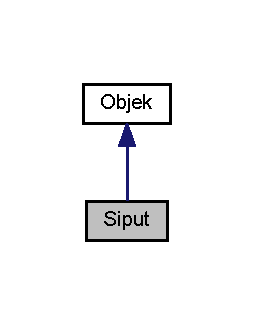
\includegraphics[width=122pt]{class_siput__inherit__graph}
\end{center}
\end{figure}


Collaboration diagram for Siput\+:\nopagebreak
\begin{figure}[H]
\begin{center}
\leavevmode
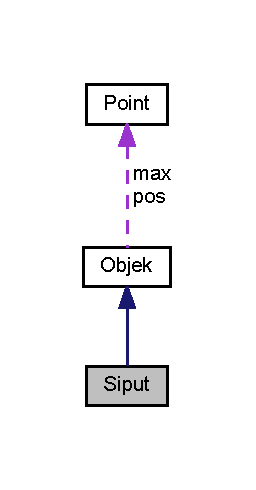
\includegraphics[width=123pt]{class_siput__coll__graph}
\end{center}
\end{figure}
\subsection*{Public Member Functions}
\begin{DoxyCompactItemize}
\item 
\mbox{\Hypertarget{class_siput_ac20b1aa07a8c41b960f5884df2bb51ef}\label{class_siput_ac20b1aa07a8c41b960f5884df2bb51ef}} 
{\bfseries Siput} (char dir, int nx)
\item 
\mbox{\Hypertarget{class_siput_a7f453530f1a4fe734b0293e413db65a2}\label{class_siput_a7f453530f1a4fe734b0293e413db65a2}} 
bool {\bfseries get\+Arah} ()
\item 
\mbox{\Hypertarget{class_siput_a64e85e42b14fd786fac8ea2245d7d18c}\label{class_siput_a64e85e42b14fd786fac8ea2245d7d18c}} 
int {\bfseries get\+Speed} ()
\item 
\mbox{\Hypertarget{class_siput_a199ef316f5226dffc9e01d417b3ee419}\label{class_siput_a199ef316f5226dffc9e01d417b3ee419}} 
void {\bfseries set\+Arah} (bool b)
\item 
\mbox{\Hypertarget{class_siput_a4eb95522cd6c685459f1296bdb6b75f5}\label{class_siput_a4eb95522cd6c685459f1296bdb6b75f5}} 
void {\bfseries set\+Speed} (int s)
\item 
\mbox{\Hypertarget{class_siput_a40de61cd661fe26389b4f53e071e44d4}\label{class_siput_a40de61cd661fe26389b4f53e071e44d4}} 
void {\bfseries move} ()
\item 
\mbox{\Hypertarget{class_siput_a5610863d03fe08a35ae1d7a3a6185d4b}\label{class_siput_a5610863d03fe08a35ae1d7a3a6185d4b}} 
\mbox{\hyperlink{class_coin}{Coin}} {\bfseries search\+Makanan} ()
\item 
\mbox{\Hypertarget{class_siput_a9c604bc409b3067bd82b0bdbaa205086}\label{class_siput_a9c604bc409b3067bd82b0bdbaa205086}} 
void {\bfseries makan} (\mbox{\hyperlink{class_coin}{Coin}} foo)
\item 
\mbox{\Hypertarget{class_siput_ae5a33b5abcda94cd574eb38dde3c681b}\label{class_siput_ae5a33b5abcda94cd574eb38dde3c681b}} 
void {\bfseries draw} ()
\end{DoxyCompactItemize}
\subsection*{Protected Attributes}
\begin{DoxyCompactItemize}
\item 
\mbox{\Hypertarget{class_siput_a21a328ffc18984b49bf2abb4f2fdfb98}\label{class_siput_a21a328ffc18984b49bf2abb4f2fdfb98}} 
bool {\bfseries arah}
\item 
\mbox{\Hypertarget{class_siput_a05d751125249fc623edf24faf13db0ea}\label{class_siput_a05d751125249fc623edf24faf13db0ea}} 
int {\bfseries speed}
\end{DoxyCompactItemize}
\subsection*{Additional Inherited Members}


The documentation for this class was generated from the following file\+:\begin{DoxyCompactItemize}
\item 
C\+:/\+Users/\+Asus/\+Documents/\+O\+O\+P/\+New folder/arkavquarium/\+Arkav\+Quarium/arkavquarium/\+Arkav\+Quarium/Siput.\+hpp\end{DoxyCompactItemize}

\hypertarget{class_submarine}{}\section{Submarine Class Reference}
\label{class_submarine}\index{Submarine@{Submarine}}


Inheritance diagram for Submarine\+:\nopagebreak
\begin{figure}[H]
\begin{center}
\leavevmode
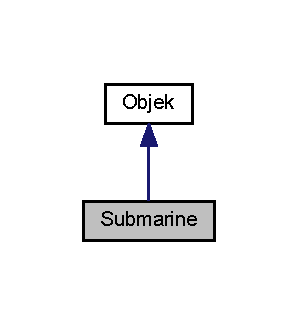
\includegraphics[width=143pt]{class_submarine__inherit__graph}
\end{center}
\end{figure}


Collaboration diagram for Submarine\+:\nopagebreak
\begin{figure}[H]
\begin{center}
\leavevmode
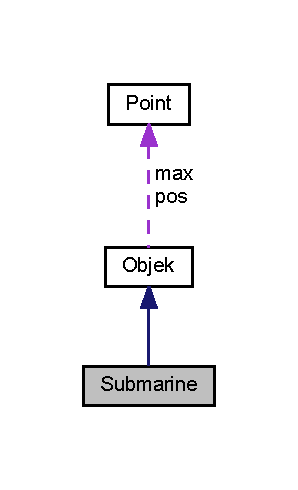
\includegraphics[width=143pt]{class_submarine__coll__graph}
\end{center}
\end{figure}
\subsection*{Public Member Functions}
\begin{DoxyCompactItemize}
\item 
\mbox{\Hypertarget{class_submarine_a082ce84d98c3bb77f4c6b37b7b722fff}\label{class_submarine_a082ce84d98c3bb77f4c6b37b7b722fff}} 
{\bfseries Submarine} (int x, int y)
\item 
\mbox{\Hypertarget{class_submarine_aa1e9de02659e527c9317af6d0735ae38}\label{class_submarine_aa1e9de02659e527c9317af6d0735ae38}} 
void {\bfseries move} (int x, int y)
\item 
\mbox{\Hypertarget{class_submarine_a8dd0ef8e7a4807af41c618785c8862e0}\label{class_submarine_a8dd0ef8e7a4807af41c618785c8862e0}} 
\mbox{\hyperlink{class_coin}{Coin}} {\bfseries search\+Makanan} ()
\item 
\mbox{\Hypertarget{class_submarine_a8f6a81112391e7d082923a0426a2f5f9}\label{class_submarine_a8f6a81112391e7d082923a0426a2f5f9}} 
void {\bfseries draw} ()
\item 
\mbox{\Hypertarget{class_submarine_aec0e6c8564323bdf9ed23da7ccf26beb}\label{class_submarine_aec0e6c8564323bdf9ed23da7ccf26beb}} 
void {\bfseries makan} (\mbox{\hyperlink{class_coin}{Coin}} foo)
\item 
\mbox{\Hypertarget{class_submarine_a61ee6583f51781411784f43cfd20f2b2}\label{class_submarine_a61ee6583f51781411784f43cfd20f2b2}} 
void {\bfseries set\+Position} (int x, int y)
\end{DoxyCompactItemize}
\subsection*{Protected Attributes}
\begin{DoxyCompactItemize}
\item 
\mbox{\Hypertarget{class_submarine_a12e519e706f360e36f8b86e47fa9e754}\label{class_submarine_a12e519e706f360e36f8b86e47fa9e754}} 
std\+::string {\bfseries image}
\item 
\mbox{\Hypertarget{class_submarine_a7d48bdb23e694916d3c4ebf6891926b0}\label{class_submarine_a7d48bdb23e694916d3c4ebf6891926b0}} 
bool {\bfseries arah}
\end{DoxyCompactItemize}
\subsection*{Static Protected Attributes}
\begin{DoxyCompactItemize}
\item 
\mbox{\Hypertarget{class_submarine_a921dd740564221375149cc88d40fb010}\label{class_submarine_a921dd740564221375149cc88d40fb010}} 
static const int {\bfseries speed} = 5
\end{DoxyCompactItemize}
\subsection*{Additional Inherited Members}


The documentation for this class was generated from the following file\+:\begin{DoxyCompactItemize}
\item 
C\+:/\+Users/\+Asus/\+Documents/\+O\+O\+P/\+New folder/arkavquarium/\+Arkav\+Quarium/arkavquarium/\+Arkav\+Quarium/submarine.\+hpp\end{DoxyCompactItemize}

%--- End generated contents ---

% Index
\backmatter
\newpage
\phantomsection
\clearemptydoublepage
\addcontentsline{toc}{chapter}{Index}
\printindex

\end{document}
